\paragraph{Logo}
	Figura \ref{fig:logo_aparcaCoches}
	\begin{figure}[h]
		\centering
		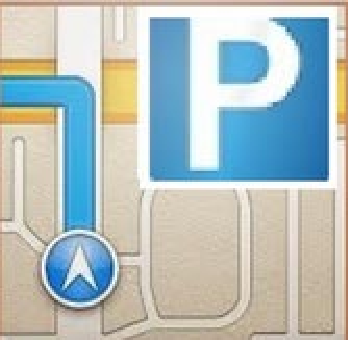
\includegraphics[scale=.6]{./estudioDeMercado/analisisDeLaOferta/source/logo_aparcaCoches}
		\caption{Logo AparcaCoche}
		\label{fig:logo_aparcaCoches}
	\end{figure}

\paragraph{Descripci�n}
Aparcacoches es una aplicaci�n donde podr�s recordar autom�ticamente la posici�n del coche aparcado y llegar hasta �l sin ning�n tipo de problema. Adem�s podr�s anotar referencias adicionales para localizarlo y obtener informaci�n del punto donde te encuentras de forma instant�nea. B�sicamente con la aplicaci�n Aparcachoches podr�s:
\begin{itemize}
	\item Guardar la posici�n de tu coche aparcado
	\item Ver en el mapa tu posici�n actual y la del coche
	\item Trazar la ruta m�s cercana entre tu posici�n y la del coche
	\item Anotar referencias adicionales sobre el aparcamiento de tu coche: Parking, plaza de parking, etc
	\item Obtener direcci�n y coordenadas de tu posici�n actual, del coche y de cualquier punto del mundo
	\item Obtener distancias entre tu coche y tu posici�n actual
	\item Cambiar preferencias de visualizaci�n en el tipo de mapa, animaciones de posicionado, c�lculo de coordenadas, c�lculo de distancias, etc.
	\item Recibir ayuda sobre cualquiera de estas funciones anteriores a trav�s de unas instrucciones bien detalladas en la aplicaci�n
	\item �Ya no olvidar�s jam�s donde aparcaste tu coche!
\end{itemize}


\paragraph{Precio}
	Gratis

\paragraph{Plataformas}
	\begin{itemize}
		\item Android
	\end{itemize}
	
\paragraph{Link}
	\begin{itemize}
		\item \url{https://play.google.com/store/apps/details?id=com.lumibasqui.mapas}
	\end{itemize}
		